% ============================ Enrico Ribiani 16-03-2021 ====================================================================
% Base per i documenti  
\documentclass[12pt]{article}
% ------------ pacchetti necessari ----------------
\usepackage[a4paper, total={6in, 8in},margin=1in]{geometry} % formattazione decente della pagina
\usepackage{graphicx}                            % need for figure
\usepackage{amsmath}
\usepackage{amsfonts}                            % if you want the fonts
\usepackage{amssymb}                             % if you want extra symbols
\usepackage{graphicx}  
\renewcommand{\figurename}{Figura}  
\renewcommand{\contentsname}{Indice}                        % need for figures
\usepackage{mathptmx}
\usepackage{float}                               % serve per mettere tabelle e immagini dove si vuole 
\usepackage[utf8]{inputenc}
\usepackage{textcomp}
\usepackage[hang,flushmargin,bottom]{footmisc}   % footnote format
\usepackage{fancyhdr, lastpage}
\usepackage{titlesec}
\usepackage[table,dvipsnames]{xcolor}
%\pagestyle{fancy}
%\renewcommand{\headrulewidth}{0pt}
%\renewcommand*\contentsname{Indice}
\titleformat{\section}{\normalsize\bfseries}{\thesection.}{1em}{}	% required for heading numbering style
\titleformat*{\section}{\Large\bfseries}
\titleformat*{\subsection}{\large\bfseries}
%\usepackage{siunitx}
%\usepackage{tikz}
\usepackage{circuitikz}
\usepackage{multicol}
%\usepackage[siunitx]{circuitikz}
\usepackage{multirow}
\usepackage{tikz}
\usepackage{amsmath}
\usetikzlibrary{angles,quotes}
\usepackage{placeins}

\usepackage{wasysym}
%===================links=================
\usepackage{hyperref}
\hypersetup{
    colorlinks=true,
    linkcolor=darkgray,
    filecolor=Green,      
    urlcolor=Cyan,
    pdftitle={SAMPLE},
    pdfpagemode=FullScreen,
    }
%===================inizio pagina del titolo=================
\begin{document}
    \begin{titlepage}
    \begin{center}
% ------------------ inizio immagine logo ----------
\begin{figure}
    \centering
    
\includegraphics[scale=1.3]{/home/r1bbi/Documenti/latec/logo.png}
    
\end{figure}
% ------------------ fine immagine logo ----------
% ------------------ fine immagine logo ----------
-------------------------------------------------------------------------------------\\
\vspace{2\baselineskip}
\large Prova n°4
\hfill
\large $5^a$   AUB\\
\begin{flushleft}
    \large Enrico Ribiani\\
    \large Daniel Graziadei\\
    \large Gruppo 11\\
\end{flushleft}


\vfill

\Huge{\textbf{Raddrizzatore trifase a singola e doppia semionda }}\\
\vfill
\vfill
\large{9-3-2023}
\end{center}
%=============== fine pagina titolo ===============
\end{titlepage}
\thispagestyle{empty}
\tableofcontents
\newpage
\setcounter{page}{1}
\vskip 1cm
\section{Scopo}
Lo scopo di questa esperienza è verificare sperimentalmente tramite \textit{Multisim} i valori teorici calcolati.
\section{Raddrizzatore a singola semionda}
\subsection{Schema}
\begin{figure}[!h]
    \centering
    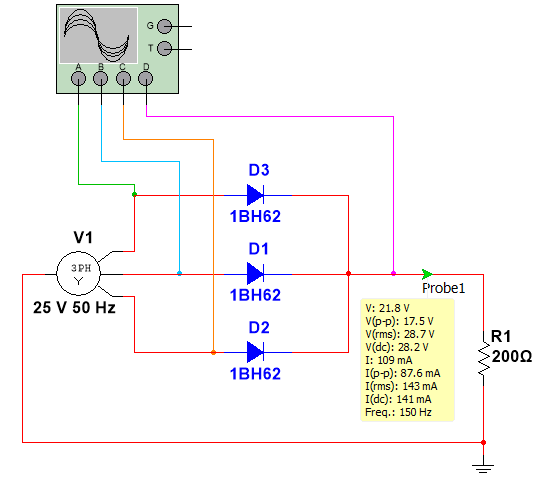
\includegraphics[scale=0.6]{schemsingsem.PNG}
\end{figure}
\subsection{Materiale e Strumenti}
\label{Materiale e Strumenti}
\begin{multicols}{2}
    \begin{itemize}
    \item Generatore a stella 25V 50Hz
    \item 3x diodo 1BH62
    \item Resistenza da $200\Omega$
    \end{itemize}
    \vfill\null
    \columnbreak
    \begin{itemize}
    \item Oscilloscopio
    \item Multimetro
    \end{itemize}
    \vfill\null
    \end{multicols}
\vspace{15pt}
\subsection{Contenuti Teorici}
Questo circuito rientra nella categoria dei convertitori \textit{a.c.-d.c.}\\
I diodi conducono solamente uno alla volta, ossia conduce solamente quello con il potenziale più alto.\\
La tensione sul carico  sarà il risultato dell'inviluppo superiore dei valori assunti dalle tre tensioni di fase.\\
\subsubsection{Descrizione della Prova}
Tramite il software \textit{Multisim} andiamo a simulare un circuito raddrizzatore trifase a singola semionda con i componenti dati.\\
Dopodichè andiamo ad osservare la tensione sul carico con l'oscilloscopio, misuriamo i valori di tensione
e corrente, quindi andiamo a confrontarli con i valori ottenuti dai calcoli, per misurare la discrepanza tra i valori di multisim e i valori calcolati, in modo da verificare sperimantalmente
i calcoli fatti.\\
\subsection{Raccolta dei dati}
\begin{figure}[!h]
    \centering
    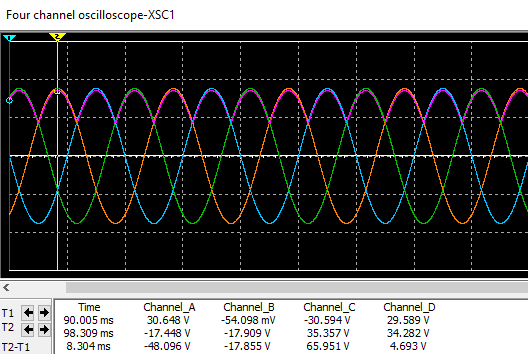
\includegraphics[scale=1]{oscsing.PNG}
\end{figure}
\subsubsection{Tabella}
\begin{table}[ht]
    \centering
    \begin{tabular}{|c|c|}
        \hline
        \rowcolor{RoyalBlue!80}     $V_{UM}$ & 35.3V\\\hline
        \rowcolor{ForestGreen!80}   $V_{AV}$ & 28.7V\\\hline
        \rowcolor{Goldenrod!80}        $I_{AV}$ & 141mA\\\hline
    \end{tabular}
\end{table}
\subsection{Calcoli}
$V_{UM}=\sqrt{2}\cdot E_2=35V$\\
$V_{AV}=1,17\cdot E_{2}=28,5V$\\
$I_{AV}=\frac{V_{AV}}{R_c}=146 mA$\\
\subsection{Analisi critica dei risultati e conclusioni}
Possiamo notare che i valori sperimentali inseriti nella tabella e i valori calcolati differiscono di 
molto poco quindi avranno una discrepanza molto piccola.\\
Possiamo dire che il circuito si comporta come ci aspettavamo.\\

\section{Raddrizzatore a doppia semionda}

\subsection{Schema}
\begin{figure}[!h]
    \centering
    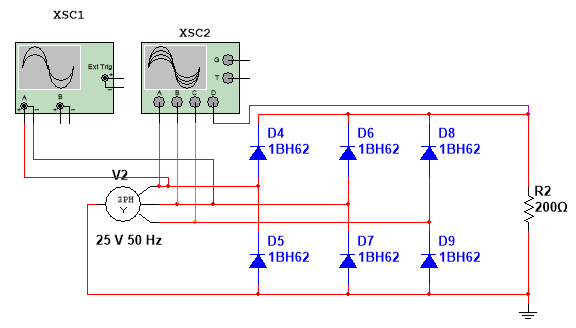
\includegraphics[scale=0.7]{schemdoppsem.PNG}
\end{figure}
\
\subsection{Materiale e Strumenti}
\label{Materiale e Strumenti}
\begin{multicols}{2}
    \begin{itemize}
    \item generatore a stella 25V 50Hz
    \item 6x diodo 1BH62
    \item Resistenza da $200\Omega$
    \end{itemize}
    \vfill\null
    \columnbreak
    \begin{itemize}
    \item Oscilloscopio
    \item Multimetro
    \end{itemize}
    \vfill\null
    \end{multicols}
\vspace{15pt}
\subsection{Contenuti Teorici}
Rispetto al raddrizzatore a singola semonda vengono usati tre diodi in più in modo da sfruttare entrambe
le semionde di ogni sinusoide.\\
Questa modifica porta come risultato l'aumento della tensione sul carico e la riduzione del fattore di ondulazione.\\
\subsubsection{Descrizione della Prova}
Tramite Multisim si simula un raddrizzatore trifase a doppia semionda e si misurano sperimentalmente
alcune grandezze precedentemente calcolate.\\ Si confrontano poi i due valori in modo da verificare se il circuito
reale si comporta effetivamente come previsto.

\subsection{Raccolta dei dati}
\begin{figure}[!ht]
    \centering
    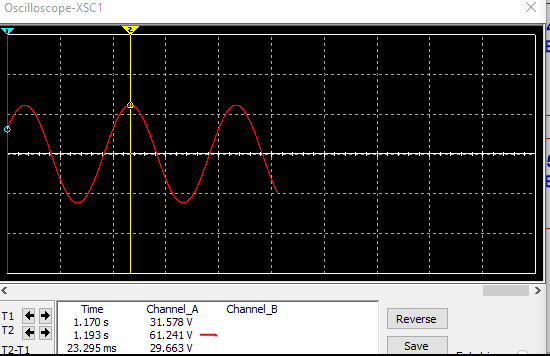
\includegraphics[scale=0.4]{oscdopp1.PNG}
\end{figure}

\begin{figure}[!ht]
    \centering
    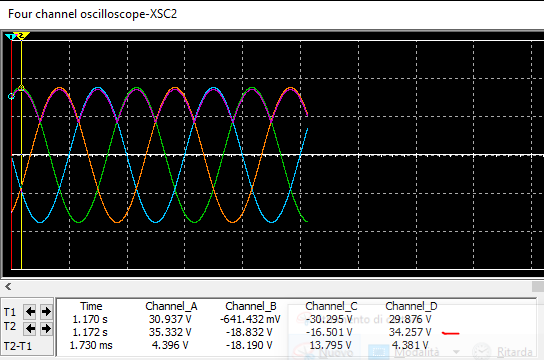
\includegraphics[scale=0.5]{oscdopp2.PNG}
\end{figure}

\subsubsection{Tabella}
\begin{table}[ht]
    \centering
    \begin{tabular}{|c|c|}
        \hline
        \rowcolor{RoyalBlue!80}     $V_{UM}$ & 61.24V\\\hline
        \rowcolor{ForestGreen!80}     $V_{AV}$ & 58.48V\\\hline
        \rowcolor{Goldenrod!80}     $I_{AV}$ & 0,3A\\\hline
    \end{tabular}
\end{table}
\subsection{Calcoli}
$V_{UM}=\sqrt{2}\cdot\sqrt{3}\cdot E_2=61,23V$\\
$V_{AV}=0,955\cdot V_{UM}=58,5V$\\
$I_{AV}=\frac{V_{AV}}{R_c}=0,29A$\\
\subsection{Analisi critica dei risultati e conclusioni}
Possiamo notare che i valori sperimentali inseriti nella tabella e i valori calcolati differiscono
molto poco quindi avranno una discrepanza molto piccola.\\
Dal momento che la discrepanza risulta piccola circuito si comporta come ci aspettavamo e lo scopo è soddisfatto.\\
\end{document}